\chapter{Preliminaries}

%\begin{abstract}
Linked Data is becoming an increasingly popular method to publish data.
It is based on a simple set of rules and a number of widely adopted standards.
This introductory article aims at capturing the simplicity of Linked Data, and the concepts behind the related standards.
It will help the reader to understand the basic elements of Linked Data and its related technologies.
Using the example of a calendar app, we will highlight the practical advantages of using Linked Data for writing apps and publishing data in a completely decoupled way.
%\end{abstract}


\section{Introduction}
\label{intro}
Linked Data is a method to publish data on the Web, so that it can be connected to other datasets and create a Web of Data.
Four rules need to be followed in order to publish data as Linked Data~\cite{linkeddata-rules}:

\begin{enumerate}
\item Use URIs to name things
\item Use HTTP URIs so that they can be looked up
\item On lookup, provide useful information in standard formats
\item Provide links to other things
\end{enumerate}
%\todo[inline]{Was ist mit einer offenen Lizenz? Siehe 5 star data}

This chapter will describe the standards around Linked Data and their basic concepts.
Instead of focusing on completeness and technical correctness, we want to achieve an intuitive understanding in the interested but so far uninformed reader.
We refer to more comprehensive primers and the technical specifications in each section, so that the reader interested in more details can further deepen their knowledge.

Prerequisites for this chapter are merely a basic understanding of how the Web works.
It would be helpful if the reader was exposed to some basic ideas from data management, data structures, and knowledge representation.

Throughout the chapter we will use the example of writing a calendar application.
Our app will be able to deal with different time zones:
if the user enters a meeting like \textit{"Meeting at 9am in Atlanta"} the calendar tool should be able to translate the time to the local time zone, even if the meeting is being entered in Istanbul and shared with participants in Athens.

The chapter is structured as follows:
Section~\ref{semanticweb} explains the connection between Linked Data and the Semantic Web Vision.
Section~\ref{rdf} introduces the basic notions of RDF, especially the idea of an RDF graph and RDF triples.
Section~\ref{uri} describes URIs, the basic building blocks for such triples, and how they refer to the Web.
Section~\ref{http} then discusses how the Web is used for the distributed publishing of knowledge using the HTTP standard.
Secton~\ref{rdfs} extends the very simple expressivity of RDF, and discusses how languages like RDFS, OWL, and RIF are layered on top of it.
Section~\ref{sparql} introduces SPARQL, a query language for RDF graphs.
In Section~\ref{rdfa} we then go into more detail about the question how RDF is and can be serialized,
before we devote Section~\ref{xml} to the sometimes confusing relationship of RDF and XML.
We close in Section~\ref{conclusions} with a resum\'{e} on the state of Linked Data and an outlook on current developments.

\section{Vision of the Semantic Web}
\label{semanticweb}

Linked Data and \emph{Semantic Web} are sometimes used synonymously, although these two are rather different concepts.
The Semantic Web~\cite{semanticWeb} is a movement from the \texttt{Web of Documents} to the \texttt{Web of Data}.
The intention is to develop a Web that enables humans as well as machines to interact and work on existing data in way that creates an additional value.
To achieve this the data needs to be machine understandable, human manageable, linkable and storable in a standardized way.
Linked Data is the materialized implementation of the Semantic Web vision, executed by technologies like RDF, SPARQL, ontologies and many more decribed below.

\medskip

\textbf{Further readings}:
To get to know more about the Semantic Web vision we refer to the book~\cite{swbook} or the W3C Semantic Web website at \url{http://www.w3.org/standards/semanticweb/}.

\section{RDF: The basics}
\label{rdf}

RDF is a standardized model used for representing knowledge on the Web.
Knowledge representation in general enables to separate what a system does from what it knows~\cite{brachmannKR}, i.e., to make its knowledge explicit and not simply implicit in the program.
Decoupling knowledge from a program has several advantages, for example, it allows the knowledge base to be maintained externally, so that changes in the world may not even affect the code.

In the calendar app, one approach to deal with the different time zones would be to code the information into the program itself. 
We could simply have a function that, given a country or city name, returns the offset, implemented with a lot of \texttt{switch} or \texttt{if then else} statements.
A change in the timezone of a country would require rewriting the function and recompiling the whole application.
Instead, we could externalize the knowledge about countries and cites and their time zones.
The application would then load the knowledge base whenever it is needed, and behave accordingly.

There are many different ways to represent the knowledge in a way that the application can read it.
For example, we could have a database with tables of cities and countries and associated time zones.
We could have comma separated lists of cities for each time zone.
Or we could gather a consortium and define a standard for expressing time zone information, so that different developers can independently access this knowledge in their apps.%
\footnote{For time zones, this is roughly what happened, in form of the \textit{tz database}.}

RDF provides a generic, standardized model for representing knowledge.
Generic means, that it can be used in any domain, be it time zones, geographic data, genes, books, or anything else.
Standardized means that RDF has been specified in an explicit, reimplementable way, so that everyone can create software that can correctly read and write RDF documents.

The basic notions of RDF are triples and graphs.
Triples are used to express the given knowledge, piece by piece.
Each triple is built of three elements: a subject, a predicate, and an object.
In our example, a piece of knowledge could be expressed with the following triple:

\begin{verbatim}
 Turkey timezone EET .
\end{verbatim}

The subject in this triple is \texttt{Turkey}, the predicate is \texttt{timezone}, and the object \texttt{EET}.
The triple can intuitively be understood as having the same meaning as the English sentence \textit{"Turkey is in the timezone EET."}.

A graph consists of a set of triples.
It is called a graph, because the subjects and objects can be understood as nodes, connected with directed edges labeled with the given property.
The following example graph is visualized in Figure~\ref{fig:graph}.
\begin{verbatim}
 Turkey timezone EET .
 Greece timezone EET .
 Georgia timezone GET .
 EET borders GET .
 EET offset "2"^^int .
 GET offset "4"^^int . 
\end{verbatim}

\begin{figure}
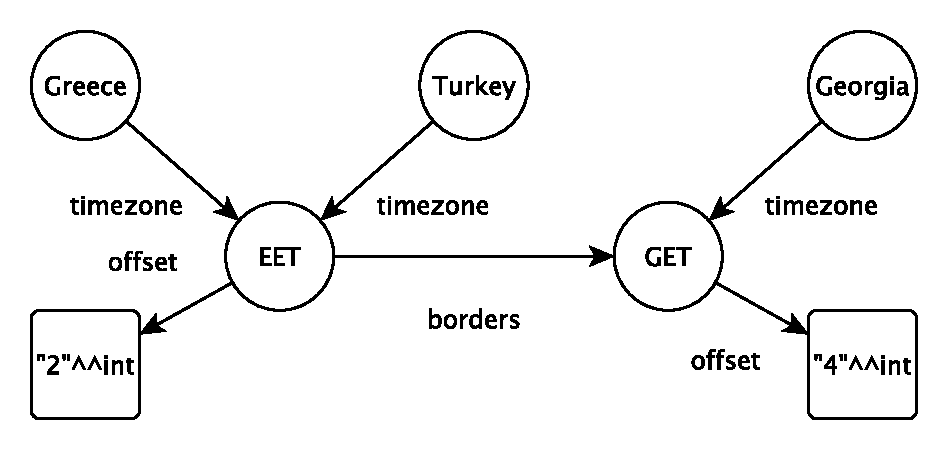
\includegraphics[width=\linewidth]{part_01/fig_graph.pdf}
\caption{Example of Linked Data used for the calender application.}
\label{fig:graph}
\end{figure}

The last two triples in the example graph demonstrate the use of literal values in the object position: instead of a named node, that refers to an entity, we have a typed literal value.
The type in this case is \texttt{int}, which means that the values should be interpreted as integers.
The types available in RDF cover numbers, strings, booleans, dates, time durations, URIs, XML, and others.

\medskip

\textbf{Further readings}:
If you want to get deeper into the formalisms behind RDF have a look at the the RDF specification~\cite{rdf-spec}, 
the RDF primer~\cite{rdfprimer}, 
the specification for XSD datatype~\cite{xsd-part2}.
Relevant concepts we did not introduce are blank nodes, reification, named graphs and extensible datatypes~cf.~\cite{namedgraphs,rdfprimer}.

\section{URIs: The words of the language}
\label{uri}

The big advantage of a graph-based model is that they can be easily be merged, by simply regarding a merger as a union of the triples in both graphs.
Many other models for knowledge representations, like tables or XML files, do not allow for such a generic merging.
But in order to provide a knowledge representation language that allows these kind of mergers, naming conflicts must be avoided.
In our example, \texttt{Georgia} refers to the caucasian country.
But now consider a second knowledge base about US states:

\begin{verbatim}
 Georgia timezone EST .
 SouthCarolina timezone EST .
 EST offset "-5"^^int .
\end{verbatim}

Since both Georgias -- the caucasian country and the US state -- are named the same, we would not be able to differentiate them.
Georgia now seems to be both in the timezone \texttt{GET} and \texttt{EST}!

To avoid this situation, all entities in Linked Data have to be referred to by unique names.
To achieve this, the names are given as URIs, most often HTTP URIs (just like websites).
The advantage of URIs is that anyone can register a prefix, and then create new names with this prefix.
The owner of the prefix is responsible for what the given name means.
So, the country Georgia could be named \texttt{http://example.org/countries\#Georgia} and the us state could be \texttt{http://example.org/usstates\#Georgia}.
As long as everyone defines new names in their own namespace only, naming conflicts can be avoided without constant coordination between all parties.

As URIs can be quite lengthy, often qualified names (or \textit{QNames}) are used.
They have the form \texttt{prefix:localName}.
Prefixes are defined locally to expand to a certain namespace, e.g., in our example we could define that the prefix \texttt{us} means the namespace \texttt{http://example.org/usstates\#}, and thus we could use the qualified name \texttt{us:Georgia} in order to refer to the complete URI \texttt{http://example.org/usstates\#Georgia}.

\medskip

\textbf{Further readings}:
To find more about the specification of URIs, see~\cite{uri} and for to get to know how to register a new URI scheme, have a look at~\cite{uri-registration}.
We did not speak about IRIs~\cite{iri} and other protocols besides HTTP, like FTP~\cite{ftp} or URN~\cite{urn}.

\section{HTTP: Distributed knowledge}
\label{http}

The second rule for publishing linked data is to use HTTP URIs.
The advantage is, that HTTP is a widely implemented protocol, that can be used over the Internet for accessing resources with a given HTTP URI.
For example, the above knowledge base could have itself the name \texttt{http://example.org/countries}.
Now a simple HTTP \texttt{GET} command like

\begin{verbatim}
 GET http://example.org/countries
\end{verbatim}

will return the knowledge base (it can be tried by entering the URI in a browser, but it is suggested for later as the result might be confusing at this point).

All entities are named with URIs, and the third rule of Linked Data asks to return information about the entity identified with a given URI when the URI is being dereferenced via HTTP.
This way, the Web can be used as vast knowledge space, where everyone can publish what they know about a given entity.

We can also use the URIs of others -- we do not have to publish URIs for all entities that we want to use ourselves.
For example, DBpedia is a widely used resource that publishes Linked Data based on Wikipedia's infoboxes~\cite{dbpedia-swj}.
DBpedia offers URIs for all entities that have a Wikipedia page.
For example, Greece' Wikipedia page is \texttt{http://en.wikipedia.org/wiki/Greece} and, based on that, DBpedia defines the URI for Greece to be \texttt{http://dbpedia.org/resource/Greece}.
If this is entered into a browser, the browser redirects the user to a Web page about Greece in DBpedia.
If a Semantic Web application would have asked, DBpedia (prefix dbpedia) would have returned the RDF data instead.

So we could replace

\begin{verbatim}
 countries:Greece tz:timezone tz:EET .
\end{verbatim}

with using the DBpedia URI for Greece and get

\begin{verbatim}
 dbpedia:Greece tz:timezone tz:EET .
\end{verbatim}

This would have the advantage that now we can learn much more about Greece: the name of the country in different languages and alphabets, its population, the name of the head of state, etc.
Suddenly, our application can use knowledge from all over the Web.

Instead of simply replacing the URI, in our case we actually state that the URIs refer to the same entity, like this:

\begin{verbatim}
 countries:Greece owl:sameAs dbpedia:Greece .
\end{verbatim}

We see, that also properties can be reused from all over the Web.
In this case we use the term \texttt{sameAs} from the OWL vocabulary, which we will look at in the next section.

One advantage of using the Web as a knowledge base is that much knowledge is already published:
whereas our knowledge bases had information on some countries, Websites like Geonames or DBpedia offer lists of cities, and in which countries or US states they are located.
So regarding the cities we mentioned in the beginning of the article, the Web already offers the following pieces of knowledge:

\begin{verbatim}
 dbpedia:Istanbul dbo:country dbpedia:Turkey .
 dbpedia:Athens dbo:country dbpedia:Greece .
 dbpedia:Atlanta dbo:isPartOf dbpedia:Georgia_(U.S._state) .
\end{verbatim}

This allows us to just reuse the knowledge about cities from the Web of Data, for very little cost.

\medskip

\textbf{Further readings}:
For a deeper introduction of the HTTP protocol have a look at the HTTP specification~\cite{http}.

\section{RDFS, OWL and others: Adding expressivity}
\label{rdfs}

RDF allows us to express triples directly.
A very powerful method is to allow for implicit triples, by using more expressive semantics than simple triples.
We have seen one example already: \texttt{owl:sameAs} states that two URIs refer to the same entity.
That means that anything we say about \texttt{dbpedia:Greece} is also true about \texttt{countries:Greece}.
So now that we learnt that \texttt{dbpedia:Athens} is in \texttt{dbpedia:Greece}, we know that it is also in our own \texttt{countries:Greece}.

A number of languages build on top of RDF and extend it with more expressive semantics.
We will look at three of them, that are standardized by the W3C: RDFS, OWL, and RIF.

RDFS is the simplest one of them.
It allows us to describe class and property hierarchies:
for example, we have found on the Web cities connected to countries resp. US states.
The connection to the country was done using the \texttt{dbo:country}, to the state with \texttt{dbo:isPartOf}.
Now we can also define that everything that is connected via the former should also be connected through the latter.
In RDFS we do that with the following triple:

\begin{verbatim}
 dbo:country rdfs:subPropertyOf dbo:isPartOf .
\end{verbatim}

Now a reasoner who follows the RDFS semantics can infer that

\begin{verbatim}
 dbpedia:Istanbul dbo:isPartOf dbpedia:Turkey .
\end{verbatim}

is true, even though it was never stated explicitly.

OWL is much more expressive regarding the description of classes and properties:
for example, we can state that every city has to be in exactly one time zone, or that nothing can be both a U.S. state and a country, which could have helped to discover the error with the two Georgias automatically.

Since RDF allows only triples, such more complex statements need to be broken down to triples.
The statement \textit{"Every city is in exactly one time zone."} translates in RDF to the following four triples:

\begin{verbatim}
x:statement1 rdf:type owl:Restriction .
x:statement1 owl:onProperty tz:timezone .
x:statement1 owl:qualifiedCardinality "1"^^xsd:nonNegativeInteger .
x:statement1 owl:onClass dbo:City .
\end{verbatim}

Although this might seem a bit daunting, in reality these kind of triples are hidden either by more high-level syntaxes (see Section~\ref{rdfa}) or query tools (see Section~\ref{sparql}).

RIF is a different beast.
Whereas OWL is an expressive language to describe classes and properties, RIF is a way to express rules of them form \textit{if\ldots{}then\ldots{}}.
In our example, we might want to state that whenever a city is part of a country or state, and the country or state has a time zone, this is also the time zone of the city. Or, using the variables \texttt{?x}, \texttt{?y}, and \texttt{?z}:%
\footnote{We will not show how the rule is represented in RDF, as this looks even worse than the OWL statement above.}

If
\begin{verbatim}
 ?x dbo:isPartOf ?y .
 ?y tz:timezone ?z .
\end{verbatim}
then
\begin{verbatim}
 ?x tz:timezone ?z .
\end{verbatim}

RDFS, OWL, and RIF can, at least in theory, be all used together.
It depends on the used tools if a given semantics is understood: some reasoners support parts of OWL (so called fragments), some support only RDFS, other RIF, and a very few claim to support interesting combinations of all three languages, and sometimes beyond.

\medskip

\textbf{Further readings}:
The whole formalism can be found in the specifications for RDFS~\cite{rdfs}, OWL~\cite{owl}, and RIF~\cite{rif},but especially at the OWL primer in this book~\cite{dl-primer}.
We did not discuss questions of how to reason and about the complexity and decidability of reasoning. 
This is a big research topic, and in the last few years, it was advanced tremendously. 
We point to the DL Handbook as an entry point into this topic~\cite{dl-handbook}.
We also did not mention the different fragments of OWL, RIF, and the differences between OWL and OWL2, which can all be found in detail in the respective standards.
Besides the languages presented here, other languages like SKOS~\cite{skos} or WSML~\cite{wsml} exist, that can define other semantics.

\section{SPARQL: Querying RDF}
\label{sparql}

So far, we have described how to express knowledge: both simple facts (with RDF) and more expressive statements that enrich the knowledge base (in the previous section).
SPARQL provides a query language for RDF knowledge bases.

For example, assume that we have all the triples we have mentioned so far in one graph that we can query via SPARQL.
Let's also assume that the system providing the SPARQL endpoint understands the semantics of RDFS, OWL, and RIF.
Now we can ask for the offset for Athens:

\begin{verbatim}
 SELECT ?offset WHERE {
   dbpedia:Athens tz:timezone ?tz .
   ?tz tz:offset ?offset .
 }
\end{verbatim}

The system will return as a result the integer $2$.

Athens is in the country Greece. We know that from the Web.
Due to the OWL subproperty triple, we also know that to be in a country means to be part of it.
Because of the RIF rule, we can infer that if something is part of something, it also has the same timezone.
Based on this, the following two triples, the first one implicit, the second given explicitly, are in our knowledge base:

\begin{verbatim}
 dbpedia:Athens tz:timezone tz:EET .
 tz:EET tz:offset "2"^^xsd:int .
\end{verbatim}

A SPARQL query describes a triple pattern (similar to the one in the \textit{if}-part of RIF),
where symbols with a leading question mark are variables.
A SPARQL processor now tries to find values for the variables, so that the whole SPARQL pattern can be fulfilled by the knowledge base.
The SPARQL processors then returns a list of all possible answers for the selected variables,%
\footnote{That is, all variables following the introductory \texttt{SELECT} keyword, in this case \texttt{?offset}.}
i.e. in this case for all values that \texttt{?offset} can have so that the SPARQL query pattern matches in the knowledge base.
Given our query pattern, the two triples above are the only match in our knowledge base, and thus the result, \texttt{"2"\texttt{\char`\^}\texttt{\char`\^}xsd:int } will be returned as the only possible value for \texttt{?offset}.

SPARQL can be regarded as the main interface to access knowledge on the Web of Data.
Currently, the usual workflow to work with Linked Data is to find and gather trustworthy data from the Web, include some knowledge created for the task or tying together the data from the Web, put it all in one knowledge base, and then use SPARQL to get answers to the queries of interest to the given task.

\medskip

\textbf{Further readings}:
To find out more about SPARQL look at the specification for SPARQL~\cite{sparql}.
We did not discuss that SPARQL is not only a query language but also a protocol of how to acccess SPARQL endpoints.
We also did not discuss other types of queries: \texttt{DESCRIBE}, \texttt{ASK}, and \texttt{CONSTRUCT}, nor the powerful features of SPARQL to count, do math, regular expressions, named graphs, etc.

\section{RDFa and Co.: Serializations of RDF}
\label{rdfa}
What is a serialization?
To send around RDF graphs through the Web, we need somehow to write them down in documents, i.e. to serialize them in a sequence of tokens.
Throughout this chapter we have used a slightly simplified, triple-based serialization, N3~\cite{n3}.
N3 has the advantage, that the triple structure of the graph is very obvious.
Although, it is widely used, it has the disadvantage of not being standard.

There are a confusing number of serializations of RDF around, mostly due to the fact that the orginally standardized serialization in RDF/XML is considered to be not very pleasing.
Soon, further syntaxes were created, some of them also in XML (like TriX~\cite{trix}), some of them not (like N3 and its constrained version N-Triples~\cite{ntriples}.
Expressions in other languages like OWL and RIF were often very cumbersome to be translated to RDF (as shown in Section~\ref{rdfs}), and thus introduced serializations of their own, like the OWL Functional Syntax~\cite{owl2}, the OWL XML presentation syntax (a serialization of OWL directly in XML, instead of going through RDF~\cite{owl3}), the RIF syntaxes~\cite{rif}, etc.
Lately, JSON became a more prominent serialization format on the Web, and standards to represent the RDF data model in JSON are being worked on~\cite{json-ld}.

%Besides serializations for pure RDF, there has been a second strand of embedding RDF in other file formats.
%One of the main use cases for RDF is to provide flexible metadata about a file.
%Embedding that metadata in the file itself has the advantage that the metadata is easier retained if the file gets moved, shared, changed, etc.
%A growing number of file formats, like Adobe's (PDF, Photoshop, etc.) allow to embed RDF~\cite{xmp}.

%The most relevant file format for the Web is obviously HTML itself, the language to describe Web pages and applications.
%The RDFa standard offers how to markup and annotate elements of a Web page with RDF.
%This allows a tool understanding RDFa to directly extract structured data out of a Website:
%a page about an event can be pulled into a calendar,
%a restaurant can be automatically filtered with the allergies of the user,
%different shopping Websites can be thrown into one knowledge base and be compared directly, etc.

\medskip

\textbf{Further readings}:
If you want to find more serializations have a look at the specifications of RDFa~\cite{rdfa}, RDF in JSON~\cite{json-ld}, and RDF/XML~\cite{rdfxml}.
Also relevant is the ongoing conversation between the communities supporting Microformats~\cite{microformats}, Microdata~\cite{microdata}, and RDFa.

\section{XML: The confusing older brother}
\label{xml}

XML became the de-facto lingua france for data on the Web and beyond.
So it was natural, that it was assumed that RDF would be build on top of XML.
But in reality, the two are very different beasts:
XML describes a tree-based model, with a single root element, that has child elements in a strict order, and, who in turn, might have further child elements, in strict orders too, all strictly hierarchical.
RDF describes a graph-based model, where the order of the edges does not matter, and that is expressed as a simple set of triples.
XML schema defines a strict grammar for the elements in an XML documents, determining if an XML file is valid or not.
RDF schemas provide additional knowledge to infer implicit knowledge from a given RDF file, and can hardly be used to check the validity of an RDF file.
It is often easier to deal with valid XML files than with RDF files, because the developer has guarantees about the structure of the file.
On the other hand, RDF files are much easier to extend: one can simply add further triples, and, as long as they don't contradict the existing triples, the knowledge simply grows.
Two RDF files can always be simply merged automatically. For XML files in general, such an operation makes no sense.

With the benefit of hindsight, forcing RDF into an XML-based serialization was bound to lead to numerous problems without gaining the hoped-for advantages.
Many of the existing XML tools and workflows were actually unable to deal with RDF/XML files, so that the existing huge pool of experience and software could not be used to kickstart the Web of Data.

Today, XML does not play a prominent role for the Web of Data anymore.
Even if it gets further used as the main serialization format for RDF, its data model and the tools used with XML are loosing relevance.
It is an open question if this might change again, or if the rich set of software and experiences surrounding the XML world can be unlocked in favor of the Web of Data -- or the other way around.

\medskip

\textbf{Further readings}:
For more information about XML, see the XML specification~\cite{xml} or the XML Schema primer~\cite{xml-primer}.

\section{Conclusions and outlook}
\label{conclusions}

RDF is increasingly becoming the standard way to share data on the Web.
Using and publishing RDF is not an academic exercise anymore.
The flexibility and extensibility of RDF, together with the possibility to merge arbitrary RDF graphs, gives it a unique advantage compared to other wide spread data models.
Confusions surrounding its several serializations, especially the ill-received standard RDF/XML-serialization, a maybe too early focus on OWL, and the late availability of SPARQL, have probably hampered uptake.
Meanwhile, simple standards like Microformats and JSON have received considerable uptake.

The advantages and the genericity of Linked Data standards are being increasingly recognized.
Instead of introducing hundreds, if not thousands of APIs and heterogeneous formats, one common data model and query language can substantially decrease costs of data integration and data reuse.

End user interfaces to the Web of Data are still missing -- but maybe they always will.
Maybe the role of Linked Data is to be background technology:
no one asks for generic interfaces for end-users to SQL databases.
Maybe the Web of Data has a similar fate.

Still several practical issues remain unresolved:
\begin{itemize}
\item In general, SPARQL is too powerful and too expensive for the Web. It is far too easy to bring a SPARQL endpoint down with a few queries.
\item The multitude of serialization formats in practical use combined with the lack of standard formats besides RDF/XML hampers teaching about RDF and its uptake.
\item For a number of wide-spread use cases, no standards or even widely acknowledged best practices exist: how to express numbers with units, especially imperial units? How to express data that was valid at a given point in time? How to express time spans? How to deal with numerical precision? How to work with simple geographical and temporal reasoning, like inclusion?
\item The current standards allow fine-grained provenance information only through reification, a method, that is often strongly discouraged for several reasons.
\item The semantics break down under inconsistencies. There is currently no accepted way to deal with diversity in knowledge bases, even though this will play a crucial role on the Web. This ties in with questions of trust that have not yet been sufficiently tackled: given diverse data about an entity, maybe even contradictions, how to choose which sources to trust? How to make this trust transferable to the user?
\end{itemize}

The Web of Data, as part of the Web, is getting increasingly tangled with all aspects of our lives.
The growing number of intelligent apps and devices in our environment will have an ever-growing need to communicate with each other.
Imagining a future where our calendar app can support the flight finder app by restricting the departure and arrival times based on our agenda and the locations of our meetings and the airport, has become much easier today than it used to be only a few years ago.
Such a future is much easier to achieve when the applications and devices can all communicate in the same common and standard data model, and using the same interfaces.

